\documentclass[tikz,border=10pt]{standalone}
\begin{document}
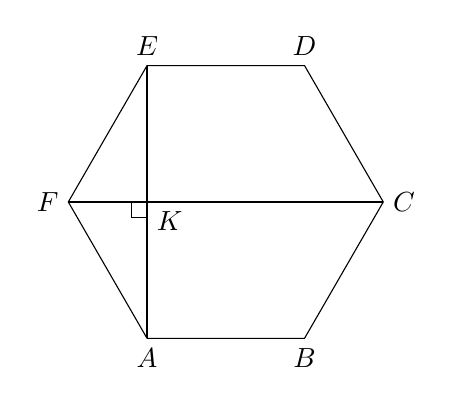
\begin{tikzpicture}
    \coordinate (A) at (-1, -1.732);
    \coordinate (B) at (1, -1.732);
    \coordinate (C) at (2, 0);
    \coordinate (D) at (1, 1.732);
    \coordinate (E) at (-1, 1.732);
    \coordinate (F) at (-2, 0);
    \coordinate (K) at (-1, 0);

    \draw (A) -- (B) -- (C) -- (D) -- (E) -- (F) -- (A);
    \draw (F) -- (C);
    \draw (E) -- (A);

    \draw (-1.2, 0) -- (-1.2, -0.2) -- (-1, -0.2);

    \node[below] at (A) {$A$};
    \node[below] at (B) {$B$};
    \node[right] at (C) {$C$};
    \node[above] at (D) {$D$};
    \node[above] at (E) {$E$};
    \node[left] at (F) {$F$};
    \node[below right] at (K) {$K$};
\end{tikzpicture}
\end{document}
